\chapter{Design Consideration}
\vspace{-5 mm}
In this chapter the system is designed with a top-down approach. First a use-case of the functionalities in the system is described, in order to give an overview of what the system must be able to do. Hereafter, constraints set by time limitations as well as a focus on the main scope of the project, in regards to the prototype, are considered. Based on the use-case description and the prototype constraints the requirements for the system's prototype are listed.
\vspace{-4 mm}
\section{Use-case design}
To give an overview of what the system should be able to do, a UML use-case diagram is used. The use-case diagram is made, where the controller is the system, because, it will be the master in this system. The actors is the external sensors and systems, that the controller is connected to. The use cases consists of the main functionalities used by the controller. See the diagram on \figref{fig:usecase}. 
%\fxnote{Is it use case or use-case}
\vspace{-3 mm}
 \begin{figure}[H]
	\centering
	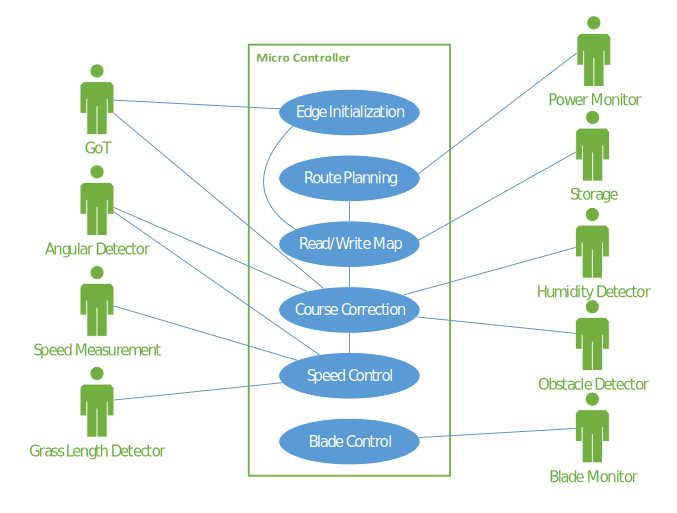
\includegraphics[scale=0.8]{figures/P5UseCase.pdf}
	\caption{Use-Case Diagram}
	\label{fig:usecase}
\end{figure}

\noindent
The system, inside the controller, have 5 main functionalities and is affected by 7 different actors.


\subsection{Main functionalities}

\textbf{Edge initialization}:
The \textit{Edge initialization} gets input from the \textit{GoT} system. The purpose of this function, is to calibrate the system to a new lawn. The function is making a map of the lawn and its edges: it locates all the areas, where the lawn shall be mowed and where the lawn mower shall not drive. This is done, by taking the system, with the \textit{GoT} system's transmitter, along these edges. From the information about all the edges, the map is created and thereafter the map is saved through the \textit{Read/write map} function.

\textbf{Route planning}:
The \textit{Route planning} gets input from the \textit{GoT} system and the \textit{Power monitor}. The purpose of this function, is to make the most suited route for the lawn mower. The route is made from the information about where the lawn mower starts, the map of the lawn, that is made in the \textit{Edge initialization} function, and the battery level from the \textit{Power monitor}. The route has to cover the whole lawn and be as effective as possible.

\textbf{Read/write map}:
The \textit{Read/write map} gets input from the \textit{Storage}. The functionality of this function, is the communication with the storage, where the map from the \textit{Edge initialization} function, is saved. 

\textbf{Course correction}:
The \textit{Course correction} gets input from the \textit{GoT} system, the \textit{Humidity detector}, the \textit{Obstacle detector} and the \textit{Angular detector}. This function measures the surroundings of the lawn mower and makes corrections, if the route, made in the \textit{Route planning} function, cannot be followed. The function makes the lawn mower stay on the route, when the route can be followed. The \textit{Course correction} is the main function behind the movement of the lawn mower.

\textbf{Speed control}:
The \textit{Speed control} gets input from the \textit{Angular detector} and the \textit{Grass length detector}. The function purpose, is to have the lawn mower to smoothly adapt the speed depending on the grass length and the route. This function powers the motor and makes it turn, whenever the \textit{Course correction} function says so.


\subsection{Actors}

\textbf{Humidity detector}:
The \textit{humidity detector} is connected to the functionality \textit{Course correction}. This is a sensor that measures the humidity in the air. The system uses the information about the ambiant humidity level to see, whether it is too high to lawn the mown in or not, since wet grass could damage the equipment. 
%\fxnote{Is this the right reason why we have this sensor?}.

\textbf{GoT}:
The \textit{GoT} system is connected to the \textit{Course correction}, \textit{Edge initialization} and \textit{Route planning} functionalities. This system is used to get the lawn mower's position on the lawn. This position is sent to the controller, which uses the information to guide the lawn mower along its route.

\textbf{Storage}:
The \textit{Storage} is connected to the \textit{Read/write map} functionality. It uses a static storage to store the information about the map, that is made in the \textit{Edge initialization} functionality. The \textit{Storage} shall have the data saved, even if the system is turn off.

\textbf{Obstacle detector}:
The \textit{Obstacle detector} is connected to the \textit{Course correction} functionality. This sensor detects, if there are any object, that block the lawn mower's route. This sensor will make sure, that the lawn mower keeps a distance to any object, like a human or a dog that could interfere with it's route.

\textbf{Angular detector}:
The \textit{Angular detector} is connected to the \textit{Course correction} and \textit{Speed control} functionalities. This sensor measures the rotation made by the lawn mower, whether it is because of the system controlling the rotation or if the lawn mower slips. This sensor is used as a feedback, to keep the lawn mower on the route.

\textbf{Grass length detector}:
The \textit{Grass length detector} is connected to the \textit{Speed control} functionality. This sensor measure the  grass length, which affects the speed, in which the lawn mower can drive with. If the grass is long, the lawn mower has to drive slower, to make sure that it doesn't get stuck in the grass. 
%\fxnote{Is this the reason?}.

\textbf{Power monitor}:
The \textit{Power monitor} is connected to the \textit{Route planning} functionality. This sensor measures how much power  is left in the battery. This is needed, so that the lawn mower can drive back to its charging station, before the battery is empty.





%The main purpose of the system is to automatically navigate in a specific area which is confined by the \textit{edge initialization} functionality. This functionality handles the marking of the areas edges. The functionality is only used in the initialization process of the system. The concept is to only use the functionality after the GoT system has been positioned in the area. The consumer then takes the system around the edges of the grass, while the GoT system tracks its positions. It is therefore only necessary to reinitialize the system, if the GoT satellites has been moved. While the edge is being tracked, the \textit{edge initialization} uses the \textit{read/write map} functionality to store the information collected, in storage. \\\\ 
%\noindent
%The route in which the lawn mower is to navigate, in the specified area, is provided by the functionality \textit{route planning}. \textit{Route planning} uses the information, about the specific area, which is collected from the storage, to plan the most optimal route. Furthermore the \textit{route planning} needs information about the systems power level to insure the functionality is considering if the system needs charging and therefore have to return to the charging station at some point on the route.\\\\
\noindent
%The \textit{read/write map} functionality as described earlier, handles the communication with storage. Hence it stores information, received from the \textit{edge initialization} and collects information from storage when the functionality \textit{route planning} needs it. \\\\
\noindent
%To insure the system is moving with a desired speed (in a straight line and in a turn) or a speed which is fitted to the height of the grass, detected with the \textit{grass length detector}, a \textit{speed control} functionality is necessary in the system to control the motors. To insure the \textit{speed control} can deliver the desired speed an \textit{angular sensor} is utilized. \\\\
%\noindent
%The last functionality, \textit{course correction} is used when the system strays of the path calculated by \textit{route planning} or if the path gets blocked.
%The obstacle which is blocking the route is detected by the sensor \textit{obstacle detector}. Furthermore the GoT system and the \textit{angular detector} will detect if the system is not on the desired path, or if the system starts to slip. Also, if it starts to rain, which is detected by the \textit{rain detector}, the system has to return to the charging station.
%Finally, the \textit{course correction} sends the calculated data to the functionality \textit{speed control}. \\\\
%\noindent
%The overall functionalities of what the system must be able to do has been described. Now the different constraints on the system will be considered and the project prototype should be established.